\documentclass[10pt,a4paper,notitlepage,twocolumn]{article}
\usepackage[latin1]{inputenc}
\usepackage{amsmath,amsfonts,amssymb}
\usepackage{graphicx,subfigure}
\usepackage[cm]{fullpage}

\author{LISA lab, U. of Montreal}
\title{Predicting Network Latency with Graph-Inspired Models}


\begin{document}
\maketitle

\section{Introduction}

This work addresses the problem of predicting the communication latency between two network locations, or addresses, using machine learning techniques.
This task is an essential component of matchmaking applications with minimal latency.
Unlike existing methods that only generalize to unseen pairs from a pool of known addresses, typically by positioning each address in a network map, we also wish to generalize to \emph{unseen addresses}.
%
This task is inherently very noisy and while the obtained relative errors can be as high as 50\%,
our objective for matchmaking purposes is twofold: (1) to correctly predict the order of magnitude of a given connection latency, and (2) to correctly determine the fastest of two candidate connections.

Our basic approach is to model the Internet network as an undirected graph where the shortest distance between two nodes is an estimate of the latency between those locations.
While we could in principle learn both graph connectivity and edge lengths, in this work we will derive connectivity from available geographical information and learn only the edge lengths.


\section{Model}

\subsection{Tree model}

Our basic assumption is that the network topology corresponds to a graph with several interconnected hubs (highly connected nodes) and that the latency between two network locations can be approximated by the distance of the shortest path between two nodes.
Intuitively, the edges will have non-negative weights but this constraint will be lifted later.


\begin{figure}[h]
\centering
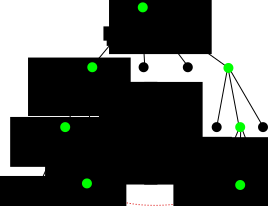
\includegraphics[width=0.8\columnwidth]{tree}
\caption{The basic graphical model is a tree of depth 3 with edges $l_i\ge0$ representing the latency between network hubs.
The overall latency between two addresses is the distance between two terminal nodes (path in green).
Shortcut edges (red) are added in the extended version.
}
\label{fig:tree}
\end{figure}


In the basic model (Figure~\ref{fig:tree}), we further assume that graph connectivity is known and corresponds to a hierarchy of geographical entities (country, region and city).
Since the resulting graph is a tree, there is a unique path between two nodes and it is easy to learn the edge lengths to minimize the squared error $C$ by solving a non-negative linear system:
\begin{equation} \label{eq:cost}
C \equiv \sum_{j=1}^N(t_j-y_j)^2
\end{equation}
for $N$ training examples with targets $t_j$, $1\le j\le N$ with
\begin{equation} \label{eq:y}
y = M\cdot l
\end{equation}
the predictions of the model and $M_{ji}=1$ if edge $i$ is part of the path linking location pair $j$ and 0 otherwise.


\subsection{Extended model}

We now extend the basic tree model to have the following properties:
\begin{enumerate}
\item It should be possible to add direct edges, or shortcuts, between important hubs to bypass the default hierarchy (e.g. red edge in Figure~\ref{fig:tree}).
\item The prediction should degrade gracefully with sparse data, e.g. a city unseen during training should inherit the average behavior of its parent region or country.
\item The model should also incorporate additional information such as physical distance, connection medium or full IP address.
\end{enumerate}

The strategy is to express the predictions as a regularized sum of $K$ terms with weight decay coefficients $\lambda_k$ and each term will be chosen to represent an aspect (feature) of the input address pair.
Equations~(\ref{eq:cost}-\ref{eq:y}) become:
\begin{equation} \label{eq:cost2}
C \equiv \sum_{j=1}^N(t_j-y_j)^2 + \sum_{k=1}^K \lambda_k ||l^{(k)}||^2
\end{equation}
\begin{equation} \label{eq:y2}
y = \sum_{k=1}^K M^{(k)}\cdot l^{(k)}
\end{equation}
where $M_{j:}^{(k)}$ represents the $k$-th feature vector of the $j$-th example, e.g. a one-hot vector representing the city of the host address, a one-hot vector representing the country combination of both addresses, or a real value giving the physical distance between the two locations.
It is easy to see that the basic tree model of Figure~\ref{fig:tree} can be recovered by this framework simply by using $K=7$ terms: \texttt{city1, region1, country1, country2, region2, city2} and a constant.
%
It is also possible to use second-order terms such as \texttt{(country1, country2)} or \texttt{(city1, city2)} to add direct edges in the graph, satisfying requirement 1 above, or other miscellaneous information fulfilling requirement 3 above.

The regularization coefficient $\lambda_k$ will effectively diminish the salience of a feature rarely present in the data (that could be spurious) by demanding that each $l_i^{(k)}$ affects a large number of training examples (equation~\ref{eq:cost2}).
For example, the correction due to a \texttt{(city1, city2)} term will be weighted by $(1+\lambda_k/n)^{-1}$ for $n$ occurences of a given city pair during training due to the regularization.
Since corrections associated with sparse data will tend to be small, the model will naturally fall back to features with a lot of training data (e.g. first-order terms), satisfying requirement 2 above.
It is important not to constrain the $l^{(k)}_i$ to be non-negative in this context because corrections to a coarse predictor may go in either direction.

Minimizing equation~(\ref{eq:cost2}) involves solving a huge sparse linear system with $N\cdot n_f$ entries, where the number of training examples $N\simeq 2\times 10^6$ and the number of input features $n_f\simeq10^{10}$ in our experiments.
A more efficient approach is to optimize each successive term $l^{(k)}$ in a greedy fashion by keeping the previous ones fixed, which makes each $M^{(k)}$ in reduced row echelon form and readily invertible.
This greedy approximation becomes exact as $\lambda_k\rightarrow 0$, eliminates the underdetermination associated with subpopulation terms (e.g. \texttt{city1} $\subset$ \texttt{country1}) and helps generalization.
This approach also makes it easier to select the hyperparameters $\lambda_k$ and to adaptively learn the parameters $l^{(k)}$ in an online setting.


\section{Experiments}

In the following experiments, we will report results using the metrics of $L_{1,2}$ errors:
\begin{equation}
L_p = \sqrt[p]{\frac1N\sum_{j=1}^N |t_j-y_j|^p},
\end{equation}
%
the relative error:
\begin{equation}
RE = \frac1N\sum_{j=1}^N \frac{|t_j-y_j|}{t_j},
\end{equation}
%
the confusion matrix $C$:
\begin{equation}
C_{ab} = \sum_{j=1}^N
\begin{cases}
1 & \text{ if } a=c(t_j),b=c(y_j) \\ 
0 & \text{ otherwise}
\end{cases},
\end{equation}
where $c(\cdot)$ denotes the class label of a given latency value as defined in Table~\ref{tab:cl_l12},
or the row-normalized version:
\begin{equation}
C'_{ab} = \frac{C_{ab}}{\sum_{b'} C_{ab'}},
\end{equation}
%
the classification accuracy:
\begin{equation}
CA = \frac{\operatorname{Tr}(C)}N
\end{equation}
%
and the ordering accuracy:
\begin{equation}
OA = \frac2{N(N-1)}\sum_{j=1}^N\sum_{j'>j}^N
\begin{cases}
1 & \text{ if } (t_j-t_{j'})(y_j-y_{j'})\ge0 \\ 
0 & \text{ otherwise}
\end{cases}
\end{equation}
which can also be defined class-wise, i.e. the sum for $OA_{ab}$ being only over $j,j'$ indices for which $a=c(t_j),b=c(t_{j'})$, and properly normalized.
The ordering accuracy corresponds to the probability of choosing successfully the fastest between to address pairs and is an important indicator of the usefulness of a model in matchmaking applications.


We conduct experiments on a dataset of $N=2,017,516$ ICMP round-trip times between wireless peers (Wi-Fi, 3G or other) collected during iOS games.
We randomly split the data into training, validation and test sets using a 8:1:1 ratio.
Table~\ref{tab:terms} shows the $K=21$ terms we have retained in our extended model.
For each term, $\lambda_k$ is chosen so as to optimize the validation $L_2$ error using the downhill simplex algorithm with initial value $\lambda_{k0}=10$.


\begin{table}
\centering
\begin{tabular}{|cl|}
\hline $L_2$ (ms) & Added Term \\ \hline\hline
330.4 & constant \\
330.0 & distance \\
328.1 & type1 \\
315.9 & type2 \\
315.4 & (type1, type2) \\
302.2 & country1 \\
293.0 & country2 \\
292.6 & same\_country \\
288.7 & (country1, country2) \\
280.5 & (country1, country2, type1, type2) \\
280.1 & region1 \\
278.9 & region2 \\
278.9 & same\_region \\
276.7 & (region1, region2) \\
276.1 & city1 \\
272.2 & city2 \\
272.2 & same\_city \\
263.9 & (city1, city2) \\
262.2 & ip1 \\
249.6 & ip2 \\
248.3 & (ip1, ip2) \\
\hline 
\end{tabular} 
\caption{Evolution of the validation $L_2$ error with each term added to our graphical model.}
\label{tab:terms}
\end{table}


We also compare our graphical model to other baselines: a constant prediction, a linear regression on the physical distance obtained via IP2Location and predicting the average latency between the two communicating countries.


\section{Results}


\begin{table*}[!ht]
\centering
\begin{tabular}{|l|c|c|c|c|c|}
\hline Model & $L_1$ (ms)  & $L_2$ (ms) & Rel Err & Class Acc & Ord Acc \\ \hline\hline
Constant prediction & 204.2 & 329.7 & 64.0\% & 38.0\% & 50.0\% \\
IP2Location & 204.1 & 329.3 & 63.8\% & 38.0\% & 57.9\% \\
Country pairs & 170.8 & 297.8 & 53.4\% & 39.8\% & 72.6\% \\ 
Graphical model & \bf 133.2 & \bf 249.6 & \bf 41.8\% & \bf 56.4\% & \bf 78.8\% \\ \hline 
\end{tabular} 
\caption{Prediction performance of the baseline models.}
\label{tab:comp}
\end{table*}



Table~\ref{tab:comp} presents the performance of the evaluated models in the latency prediction task.
The proposed model clearly outperforms other baselines.
While the obtained $L_{1,2}$ and relative errors remain relatively high, the classification accuracy (56.4\%) and ordering accuracy (78.8\%) indicate that the graphical model predictions lie in a reasonable range and suffice to determine the fastest of two addresses in the majority of cases. 



\begin{table}[h]
\centering
\begin{tabular}{|cccc|}
\hline
Class & Range (ms) & $L_1$ (ms) & $L_2$ (ms) \\ \hline\hline
1 & 0--99 & 135.2 & 234.8 \\
2 & 100--199 & 133.2 & 250.0 \\
3 & 200--299 & 135.1 & 254.5 \\
4 & 300--499 & 133.1 & 252.9 \\
5 & 500--999 & 130.9 & 247.3 \\
6 & 1000--5000 & 134.3 & 257.3 \\
\hline 
\end{tabular} 
\caption{Definition of the latency classes and their associated $L_{1,2}$ errors.}
\label{tab:cl_l12}
\end{table}


Table~\ref{tab:cl_l12} indicates the ranges used to define the latency classes.
Surprisingly, the $L_{1,2}$ errors do not vary much with the magnitude of the target.
This could indicate an intrinsic noise to the measurement process that is added to a more deterministic network-specific baseline latency.


\begin{figure}[h]
\centering
%\begin{tabular}{|rrrrrr|}
%\hline
%83 & 138 & 35 & 16 & 1 & 0 \\
%280 & 9981 & 6626 & 2012 & 320 & 33 \\
%89 & 2815 & 16844 & 14113 & 2270 & 145 \\
%41 & 827 & 5402 & 37251 & 14150 & 649 \\
%10 & 215 & 1014 & 9175 & 19320 & 1419 \\
%1 & 31 & 190 & 1002 & 3796 & 3052 \\
%\hline 
%\end{tabular} 
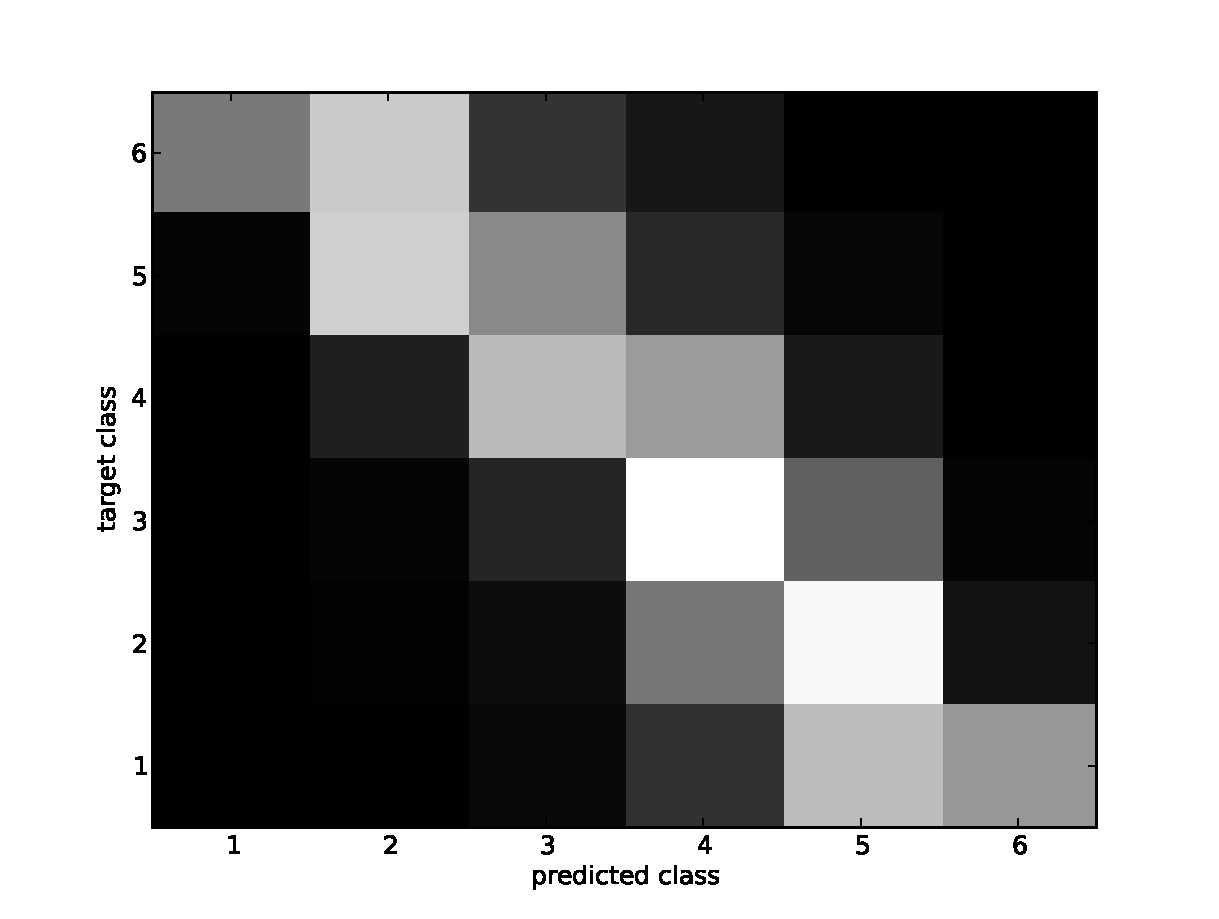
\includegraphics[width=0.8\columnwidth]{full_confusion}
\caption{Row-normalized confusion matrix $C'_{ab}$ (row: target class $c(t_j)$, column: predicted class $c(y_j)$).}
\label{fig:conf}
\end{figure}


The ability of the graphical model to correctly identify the order of magnitude of latency is also reflected in the confusion matrix, displayed in Figure~\ref{fig:conf}.
The model clearly only confuses adjacent classes around the diagonal $C'_{aa}$.

Finally, a qualitative assessment of the model performance can be obtained by plotting a few predictions randomly chosen from the test set (Figure~\ref{fig:samples}).
Again, the model correctly predicts the order of magnitude of the latency most of the time.


%\begin{table}[h]
%\centering
%\begin{tabular}{|rrrrrr|}
%\hline
%58.7\% & 79.5\% & 92.2\% & 97.4\% & 99.0\% & 99.4\% \\
%79.5\% & 63.3\% & 80.9\% & 93.7\% & 97.0\% & 98.3\% \\
%92.2\% & 80.9\% & 61.8\% & 79.5\% & 90.8\% & 94.9\% \\
%97.4\% & 93.7\% & 79.5\% & 63.7\% & 75.1\% & 87.7\% \\
%99.0\% & 97.0\% & 90.8\% & 75.1\% & 58.9\% & 75.9\% \\
%99.4\% & 98.3\% & 94.9\% & 87.7\% & 75.9\% & 59.2\% \\
%\hline 
%\end{tabular} 
%\caption{Class-wise ordering accuracy. The algorithm must select the fastest between two remote addresses belonging to classes $c_1$ (row) and $c_2$ (column).}
%\end{table}



\begin{figure}[h]
\centering
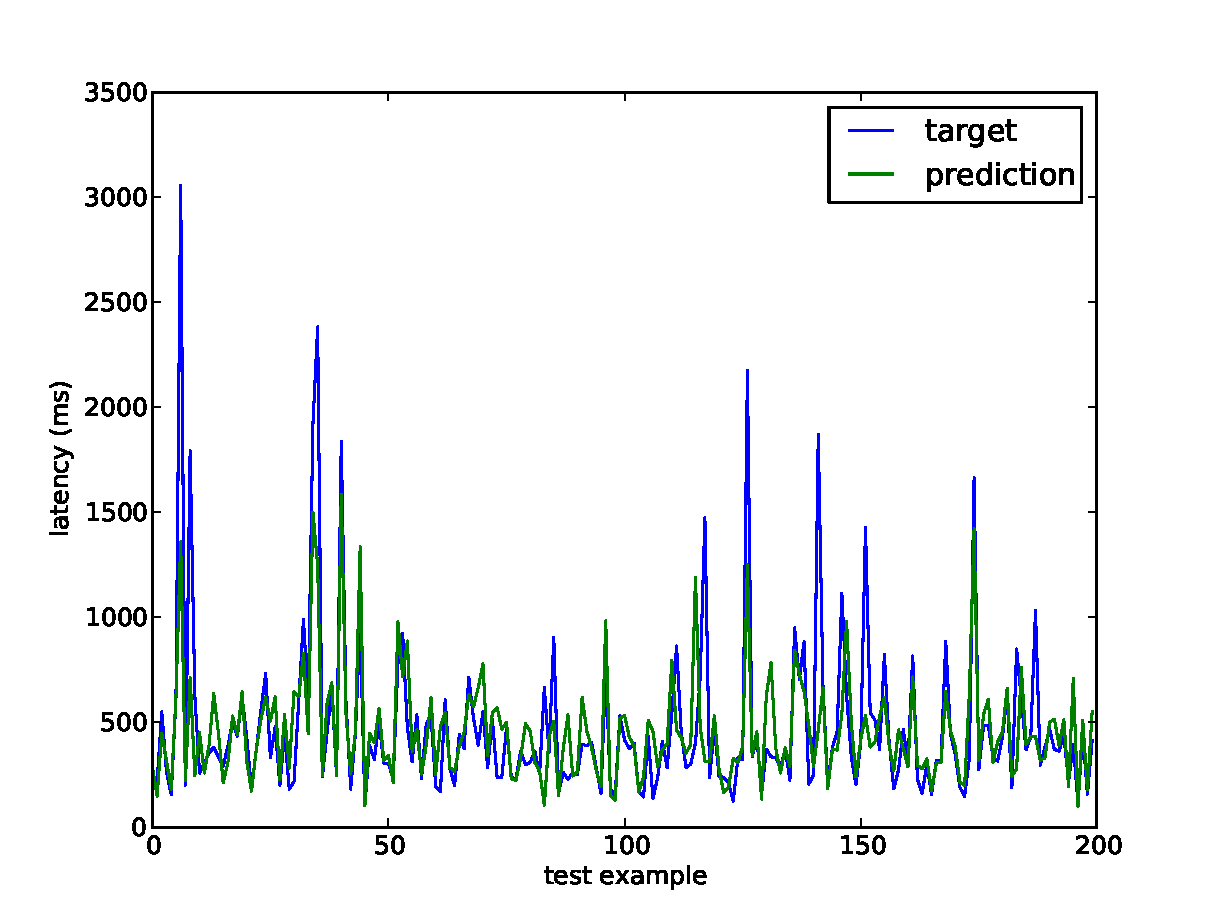
\includegraphics[width=\columnwidth]{full_samples}
\caption{A few predictions by the graphical model randomly chosen from the test set.}
\label{fig:samples}
\end{figure}


\section{Conclusion}

We have proposed a graph-inspired model to predict the communication latency between pairs of unseen network addresses.
The model obtained a test classification accuracy of 56.4\% and the $L_1$ error (133.2~ms) low variability across all ranges indicates an accurate prediction of the latency order of magnitude.
This ability translates into a high ordering accuracy (78.8\%), which is sufficiently useful to discern between candidate connections in matchmaking applications.


\newpage
\appendix
\section{Error distributions}

\begin{figure}[!h]
\centering
\subfigure[Constant prediction]{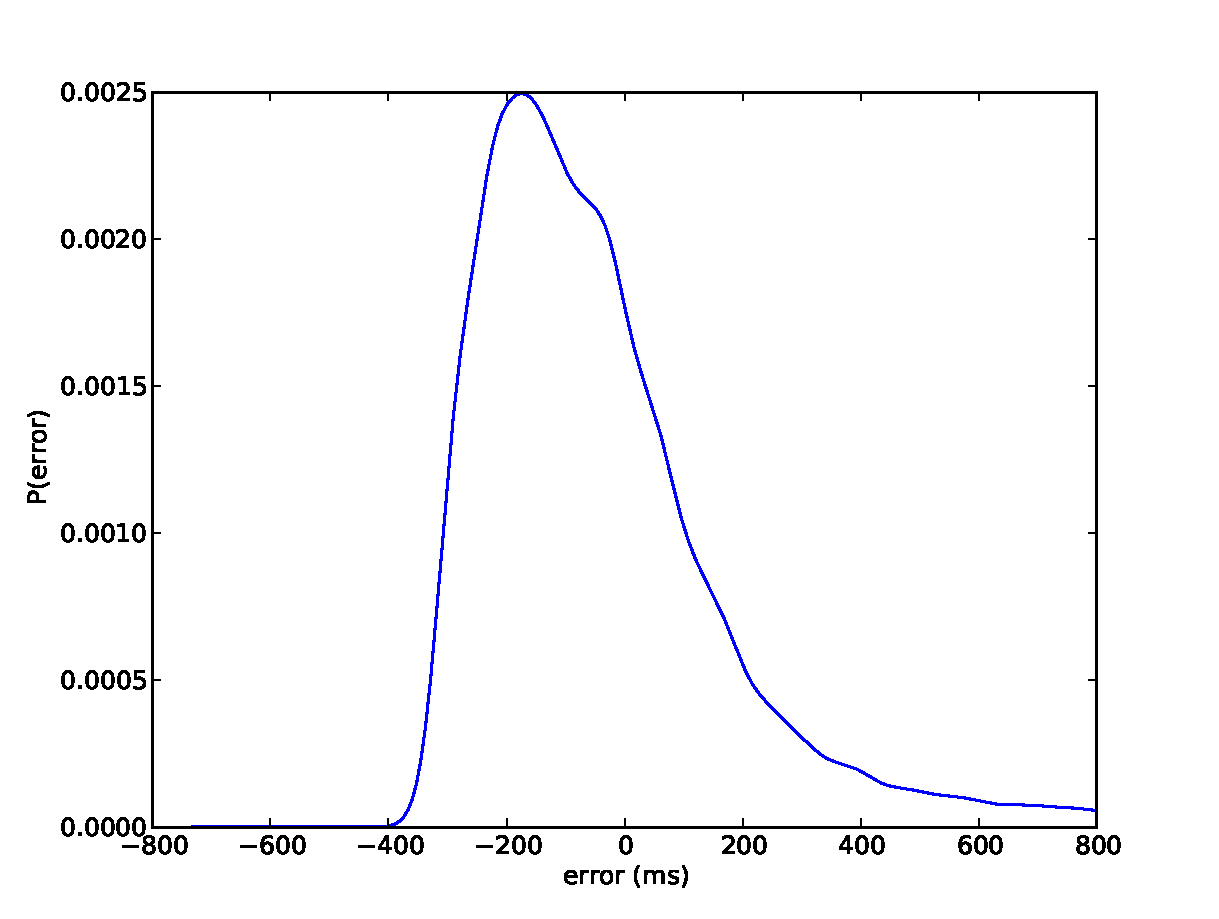
\includegraphics[width=0.75\columnwidth]{constant_dist}}
\subfigure[IP2Location]{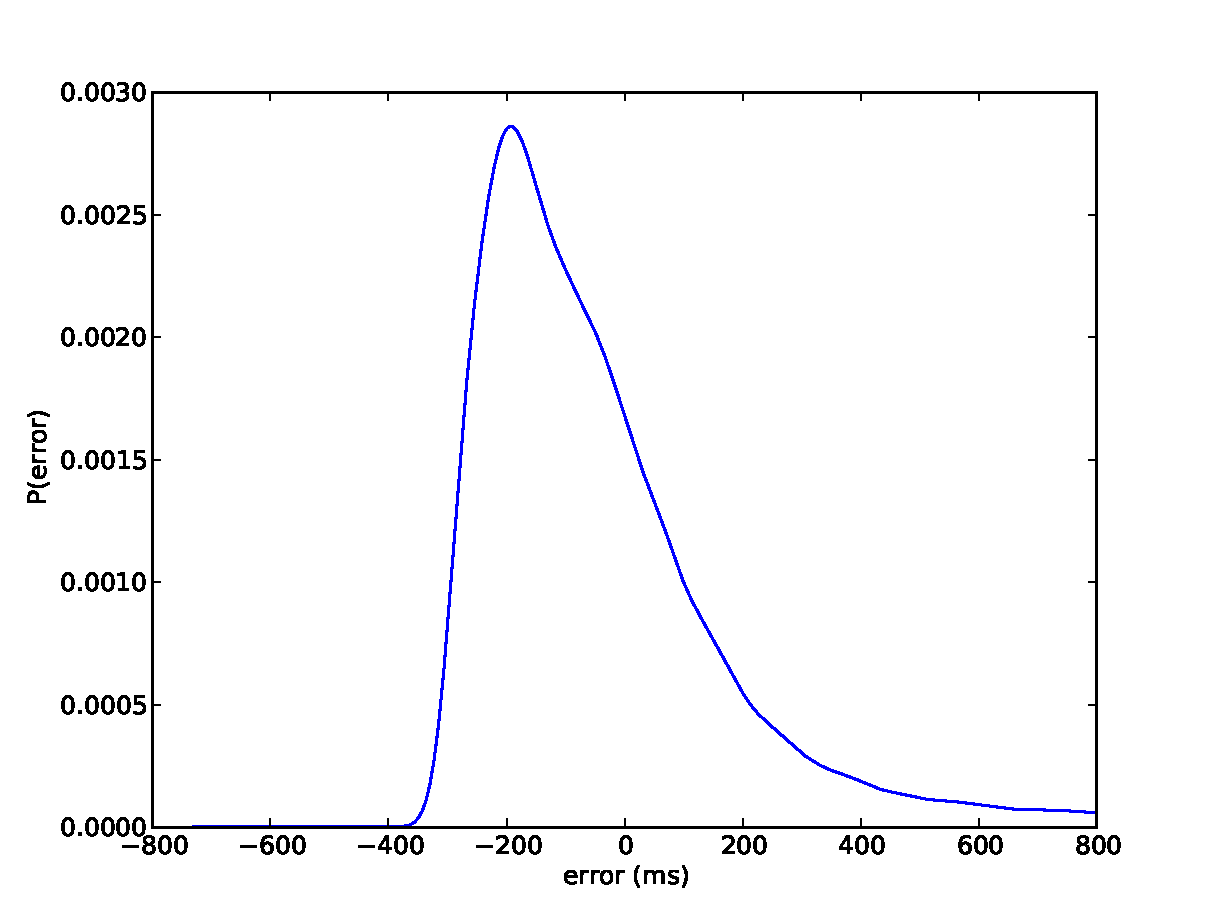
\includegraphics[width=0.75\columnwidth]{distance_dist}}
\subfigure[Country pairs]{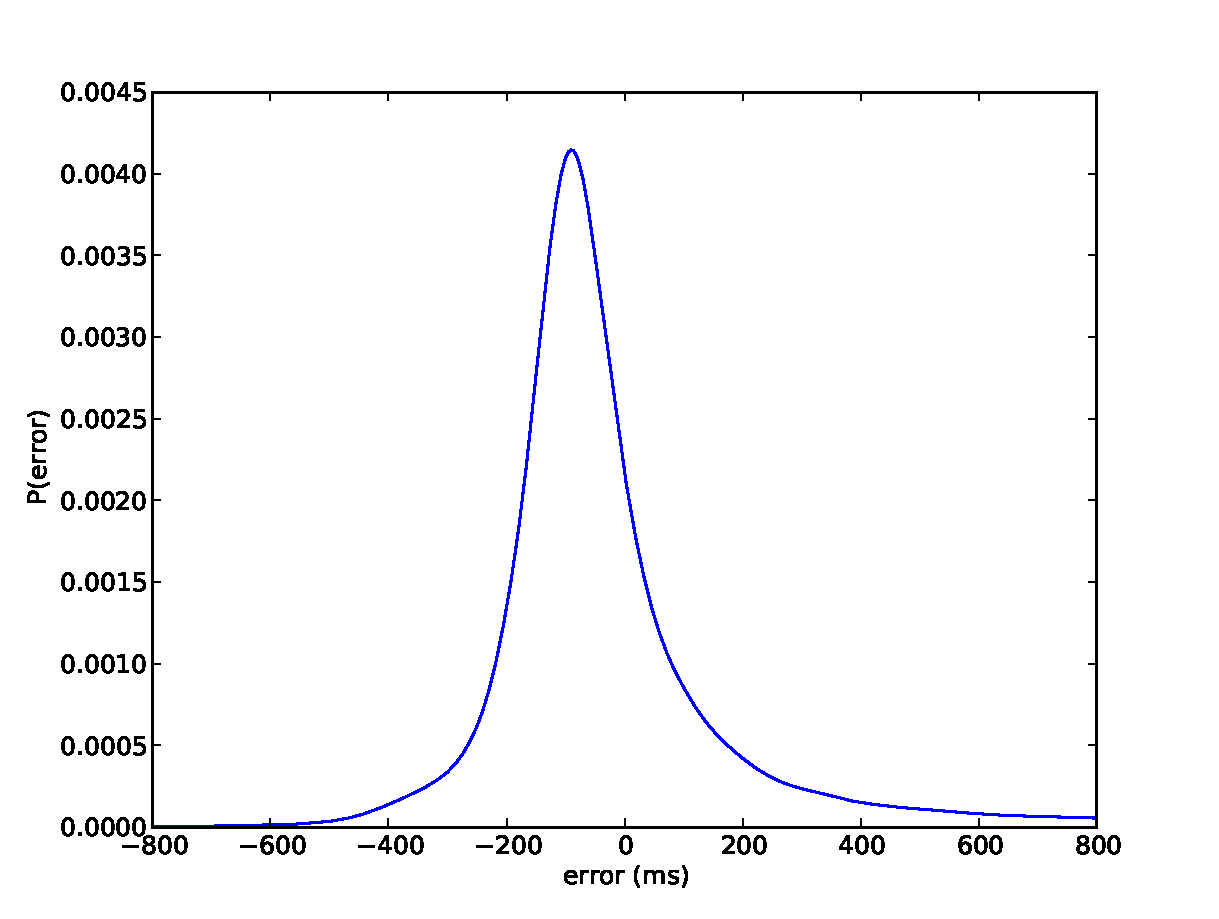
\includegraphics[width=0.75\columnwidth]{country_dist}}
\subfigure[Graphical model]{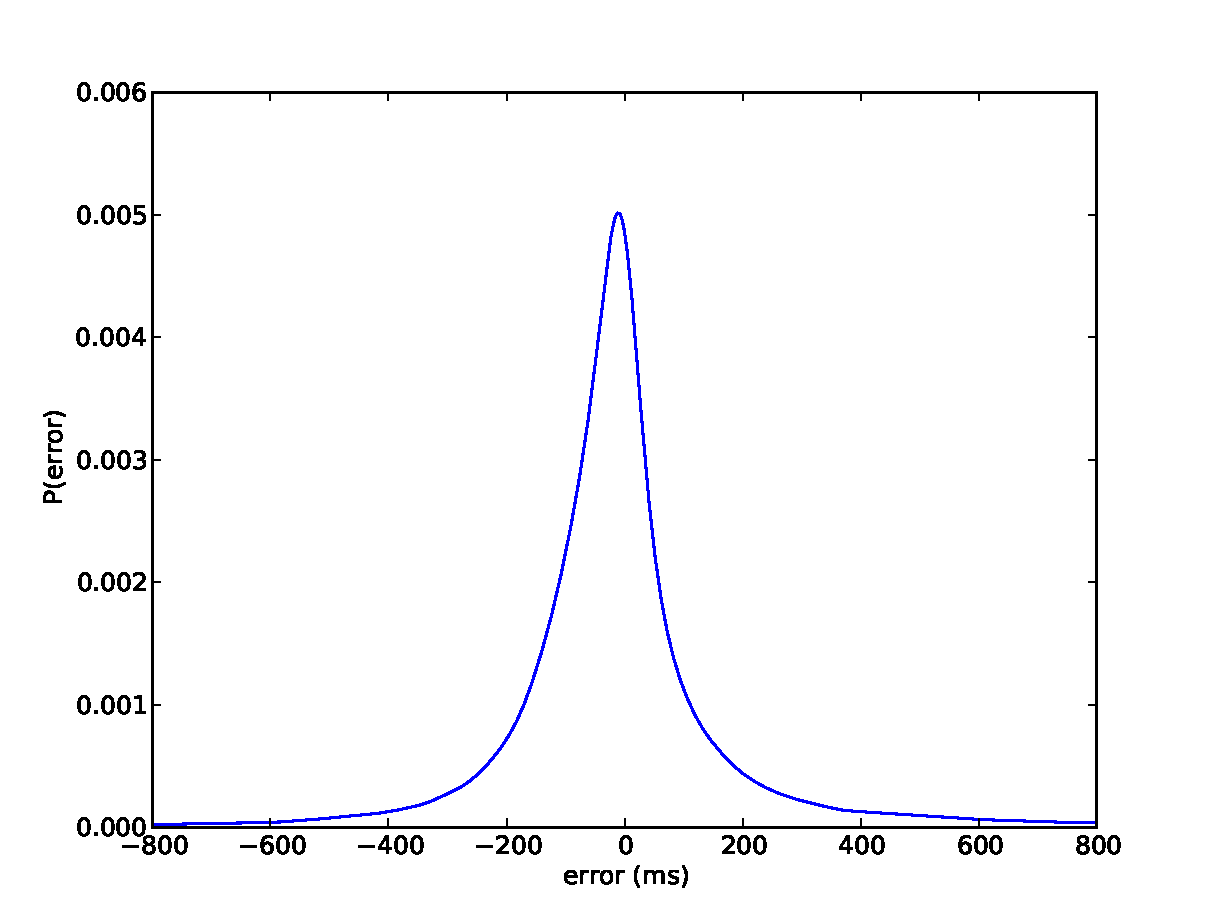
\includegraphics[width=0.75\columnwidth]{full_dist}}
\caption{Error distribution.}
\end{figure}


\begin{figure}[!h]
\centering
\subfigure[Constant prediction]{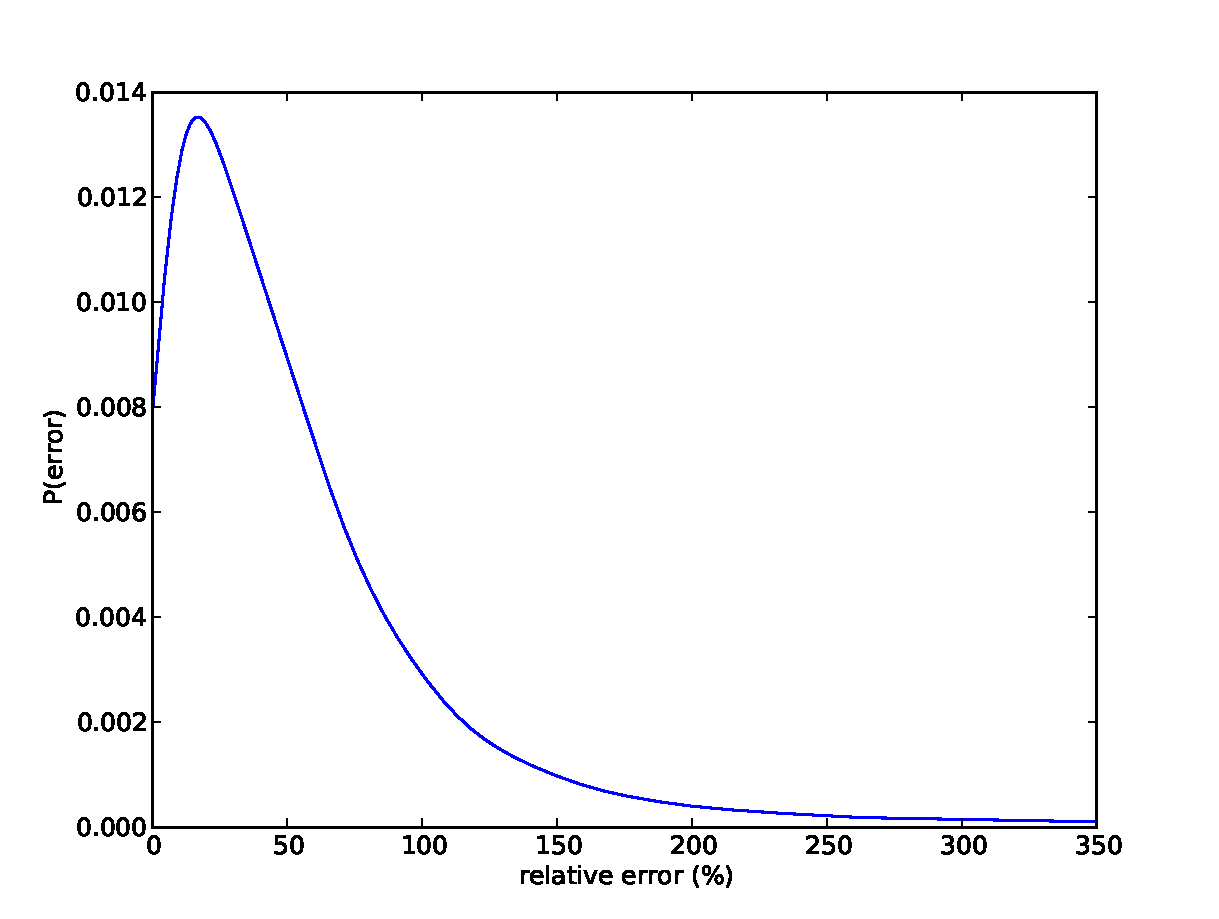
\includegraphics[width=0.75\columnwidth]{constant_rdist}}
\subfigure[IP2Location]{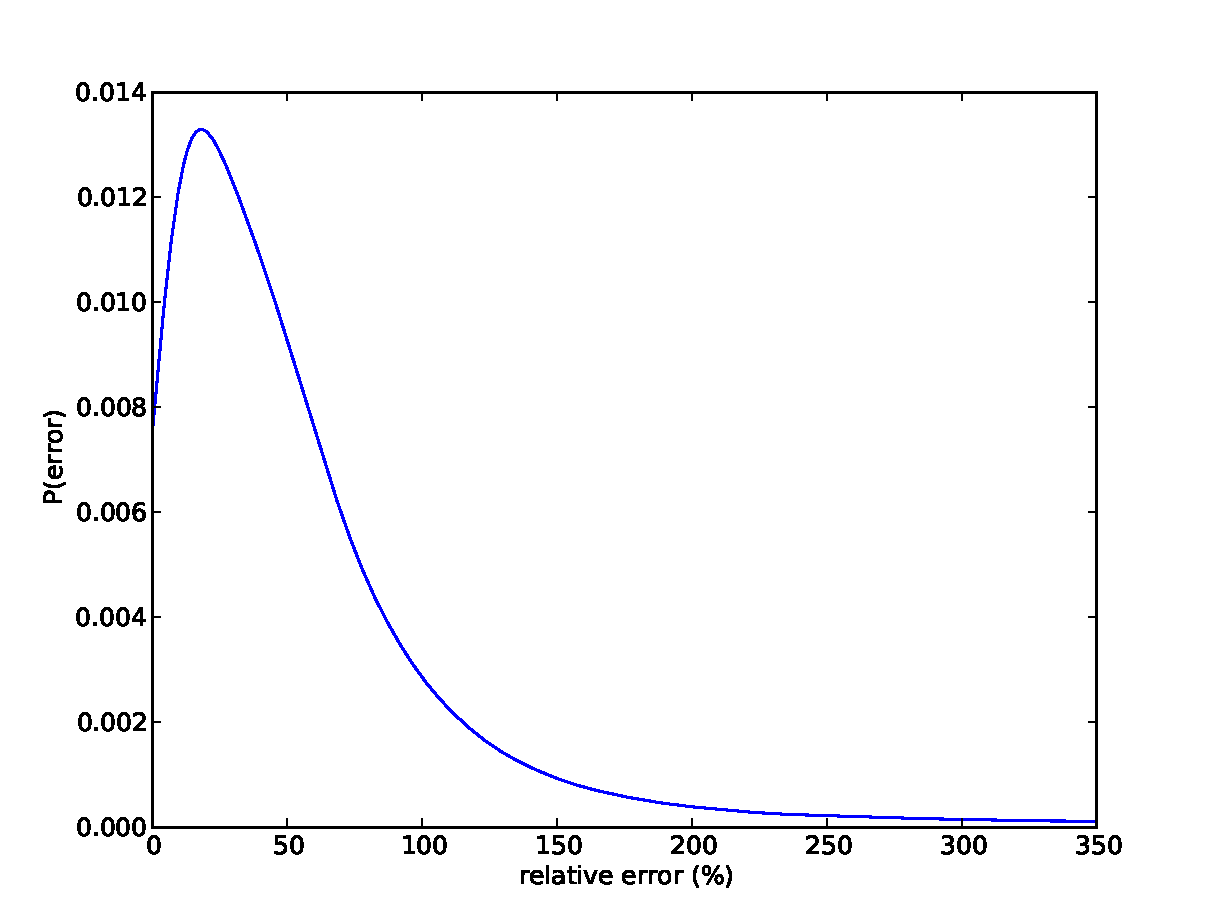
\includegraphics[width=0.75\columnwidth]{distance_rdist}}
\subfigure[Country pairs]{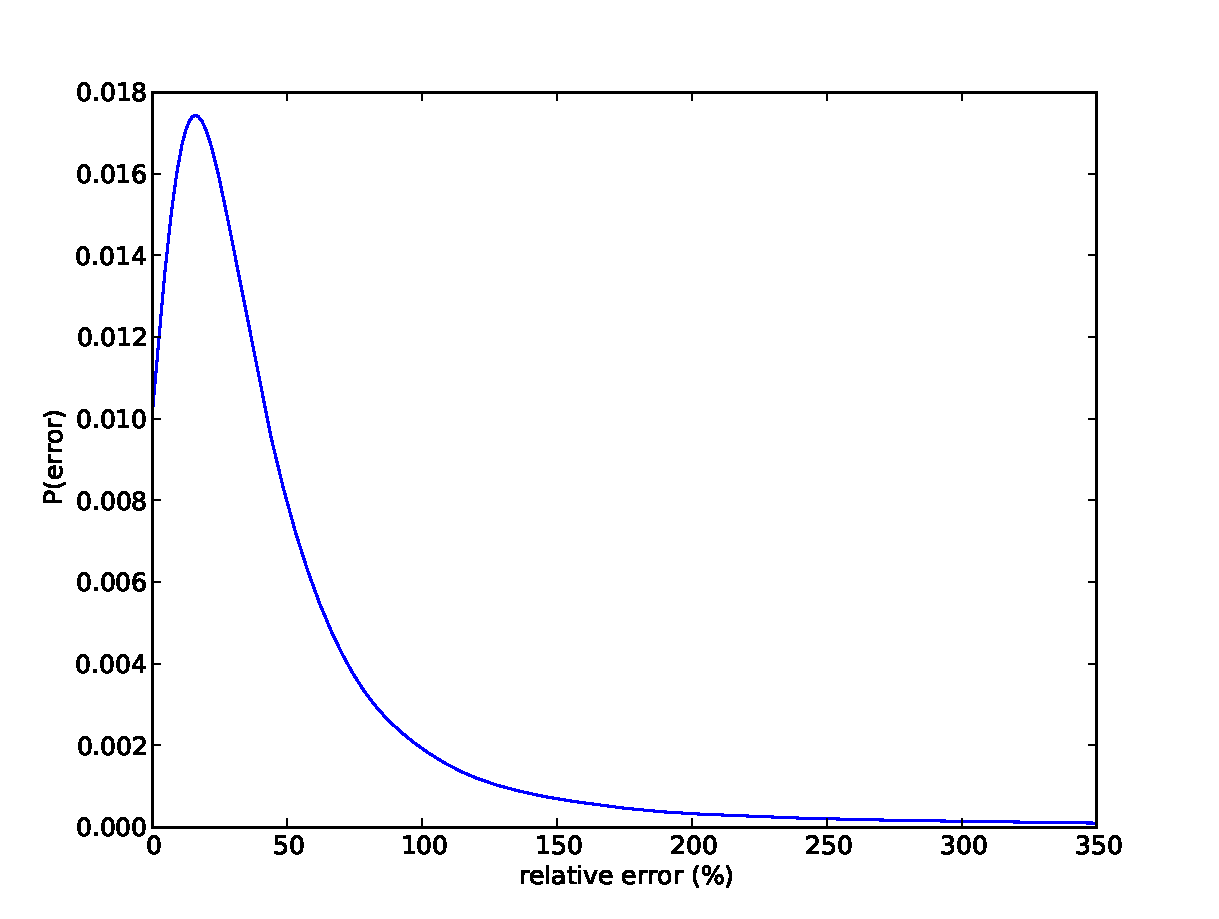
\includegraphics[width=0.75\columnwidth]{country_rdist}}
\subfigure[Graphical model]{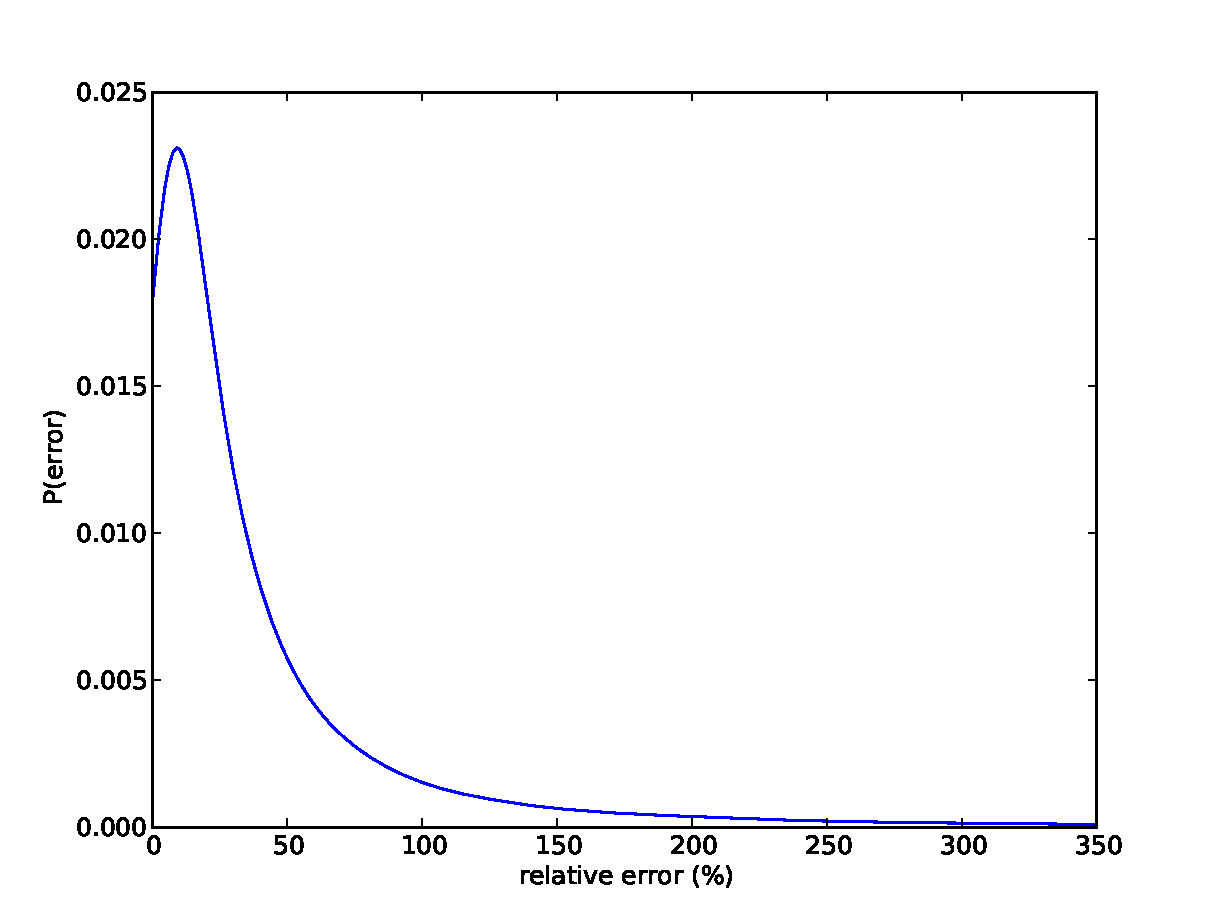
\includegraphics[width=0.75\columnwidth]{full_rdist}}
\caption{Relative error distribution.}
\end{figure}


\begin{figure}
\centering
\subfigure[IP2Location]{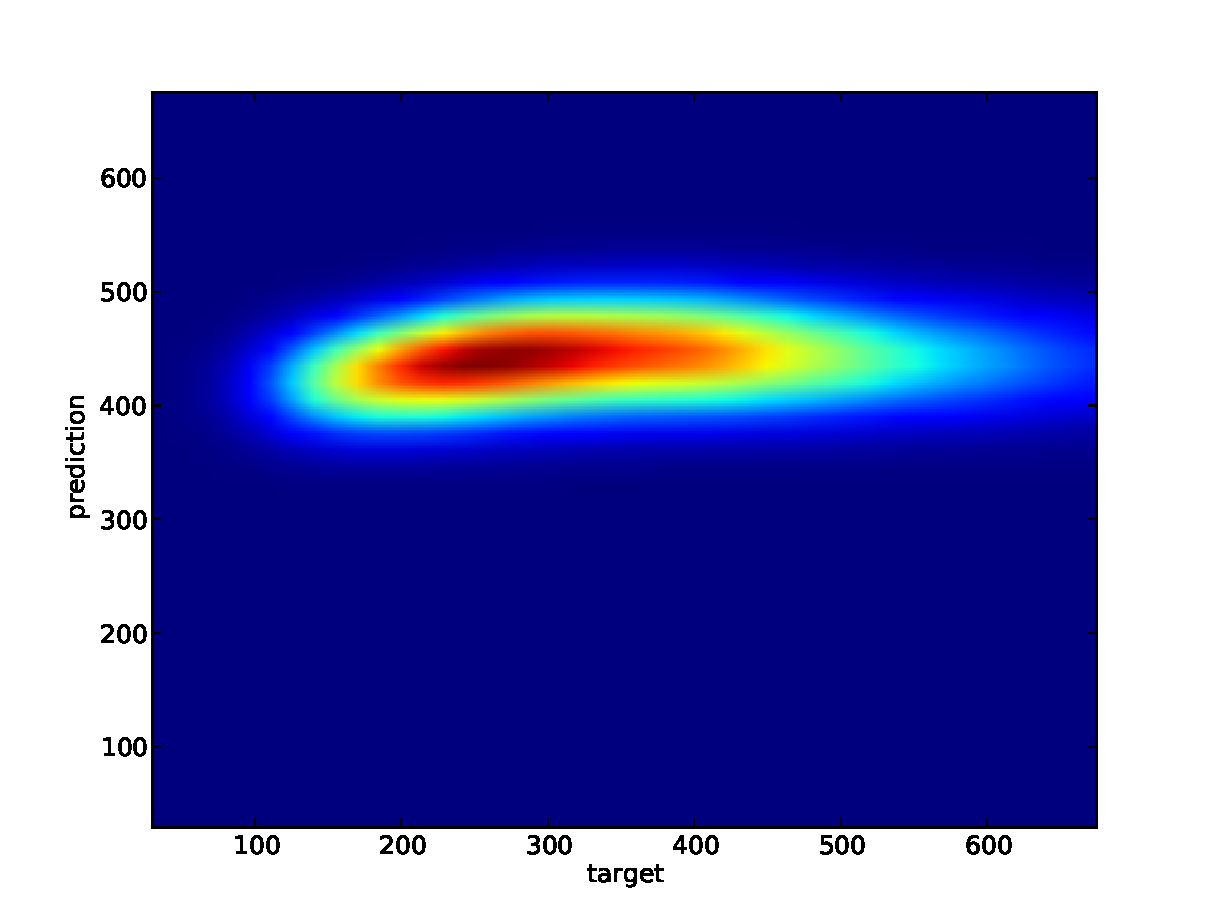
\includegraphics[width=0.7\columnwidth]{distance_2d}}
\subfigure[Country pairs]{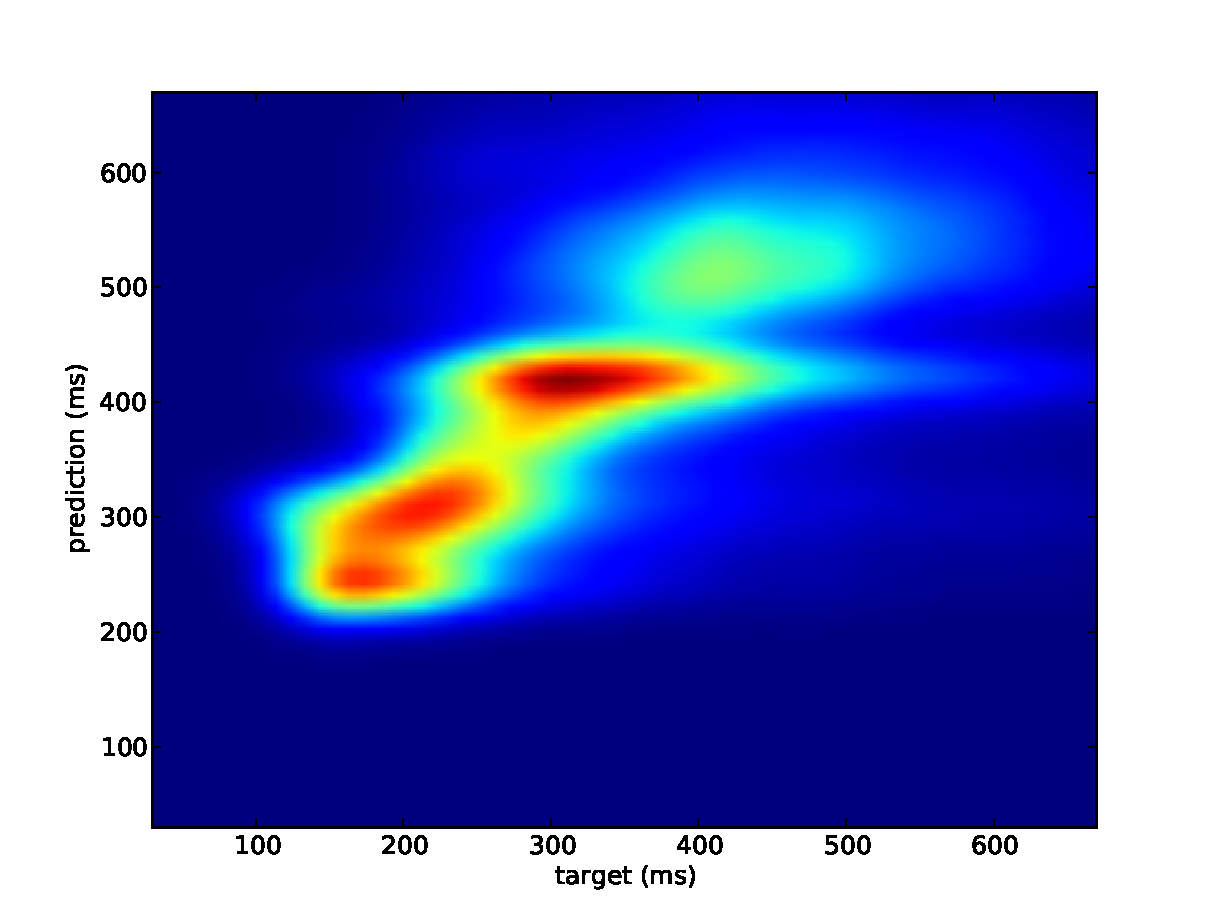
\includegraphics[width=0.7\columnwidth]{country_2d}}
\subfigure[Graphical model]{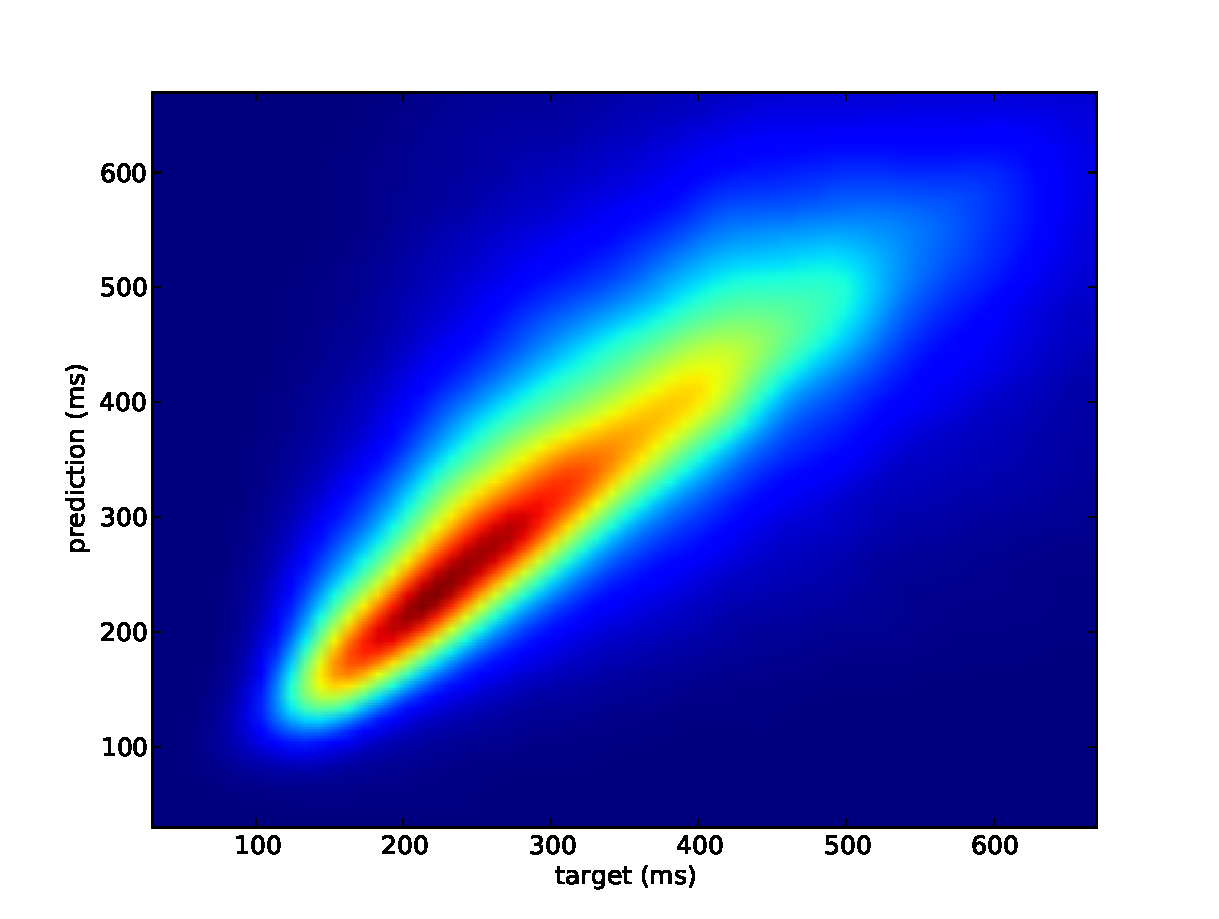
\includegraphics[width=0.7\columnwidth]{full_2d}}
\caption{Target-prediction joint distribution.}
\end{figure}

\end{document}
